
%%%%%%%%%%%%%%%%%%%%%%%%%%%%%%%%%%%%%%%%%%%%%%%%%%%%%%%%%%%%%%%%%%%%%%%%%%%%%%%%
%%%%%%%%%%%%%%%%%%%%%%%%%%%%%%%%%%%%%%%%%%%%%%%%%%%%%%%%%%%%%%%%%%%%%%%%%%%%%%%%
% OBJECTIVES %
%%%%%%%%%%%%%%%%%%%%%%%%%%%%%%%%%%%%%%%%%%%%%%%%%%%%%%%%%%%%%%%%%%%%%%%%%%%%%%%%

\chapter{Objectives} 
\label{chap:objectives} 

In this chapter, the considered objectives throughout this project are described. In addition, a temporary planning by means of Gantt Chart is included in order to detail the periods of time which have been dedicated to each of them.

\section{General objective}
\label{sec:general-objective}

The general objective of this project is composed of four clearly differentiated parts, which are described below:

\begin{itemize}
    \item To update of the design and software of the web tool Dr. Scratch to the new version of the programming language Scratch. 
    \item To develop an analysis of the bad smells detected in the Scratch projects with the support of the Dr. Scratch tool. 
    \item To implement a new model of visualization for these bad smells in order to raise awareness of their presence and importance. 
    \item To develop an assessment experiment with different teacher profiles in order to evaluate the effectiveness and impact of our study.
\end{itemize}


\section{Specific phases (and sub-objectives)}
\label{sec:specific-objectives}

In order to describe the subobjectives, in the specific phases of the project, that were necessary to achieve each part of the general objective proposed, it is important to detail what was the starting point of the project. 

At the beginning of the project, a version of Dr. Scratch already existed. This version analyzed Scratch 2.0 projects and returned different dashboards with the results. However, the work team of Scratch started to announce the launch of a new version of their language in the coming months. From this point, the specific objectives were divided into five different phases as follows:

\begin{enumerate}
    \item Documentation and training
    \begin{itemize}
        \item Documentation and training about the work context: Computational Thinking, Scratch, Dr. Scratch, bad smells in programming, Hairball, cloud tools, etc.
    \end{itemize}
    \item Update of Dr. Scratch
    \begin{itemize}
        \item To launch the existing version of Dr. Scratch: the version of Django was obsolete. It was necessary to update Django in order to start working with Dr. Scratch. 
        \item To update the code: to remove the Hairball and Kurt modules. For this objective, it was necessary the development of some scripts with the same functionality and the integration of them in the code of Dr. Scratch.
        \item To add new languages: to include the Russian language as an option in the new version of Dr. Scratch.
        \item To create a testing platform in production: to launch a first version of the Dr. Scratch update in a testing platform in Azure, during a month, and to correct possible mistakes during this period.
        \item To coordinate both versions of Dr. Scratch: to have both versions of Dr. Scratch in the same platform of Azure, working in a compatible way in the official web of Dr. Scratch.
        \item To stabilize and maintain the new version: to correct errors and to improve some functionalities.
        \item To migrate the new version of Dr. Scratch to the Google Cloud Platform.
    \end{itemize}
    \item Analysis of bad smells
    \begin{itemize}
        \item To collect data and create the files for a preliminary analysis of bad smells: in order to initiate the analysis, it was necessary to analyze a set of projects with Dr. Scratch, as well as a later process of treatment and filtering of the data.
        \item To perform an analysis of bad smells: an exhaustive analysis of the data set of analyzed projects, mainly with Pandas software. 
        \item To present the first results in the TACKLE Congress: a presentation about the results found in the general analysis of bad smells.
        \item To improve the analysis of bad smells: to collect new data for a second analysis and to improve the previous one.
        \item To develop a more specific statistical analysis of bad smells: to implement a new treatment data for a deeper analysis with the t-student process. 
    \end{itemize}
    \item Development and implementation of the bad smells model
    \begin{itemize}
        \item To improve the functionality of bad smells in Dr. Scratch: To achieve the analysis of a bigger number of cases about bad smells, such as loop dead code, backdrop naming by default, etc.
        \item To implement a new model based on bad smells in Dr. Scratch: to develop a new dashboard in which bad smells are shown in a more visual and clearer way.
    \end{itemize}
    \item Development of an assessment experiment
    \begin{itemize}
        \item To develop an assessment experiment about the bad smells model with different teacher profiles.
        \item To analyze the results of the experiment: to compare the results obtained with those of the previous analysis of bad smells, in order to check the effectiveness and impact of the study.
    \end{itemize}
\end{enumerate}



\section{Project timeline}
\label{sec:timeline-project}

This project has been carried out during two full years. In order to organize the proposed objectives temporally, we identified objectives in the short, medium and long term. In this way, the work is divided into five important phases:

\begin{itemize}
    \item Phase 1: Documentation about the context, to understand the code and fix some bugs.
    
    \begin{figure}[h]
    \centering
        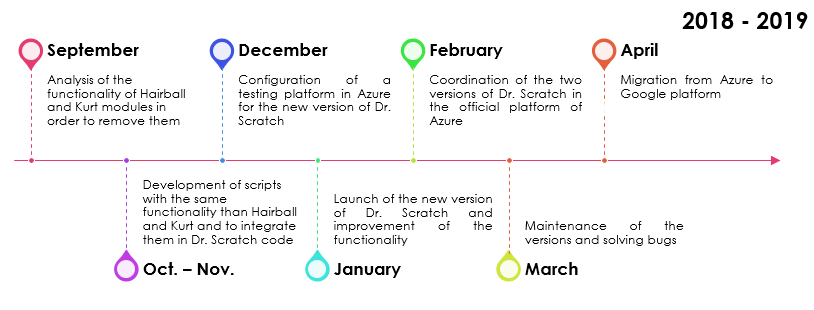
\includegraphics[width=12cm, keepaspectratio]{img/phase_1.png}
        \caption{Timeline planning for phase 1.}
        \label{fig:phase_1}
    \end{figure}

    \item Phase 2: Update of Dr. Scratch.
    
    \begin{figure}[h]
    \centering
        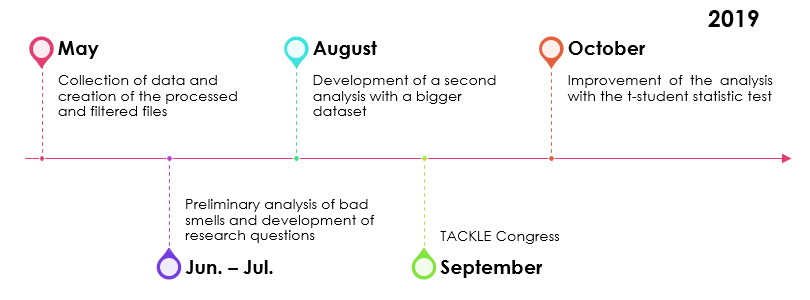
\includegraphics[width=15cm, keepaspectratio]{img/phase_2.png}
        \caption{Timeline planning for phase 2.}
        \label{fig:phase_2}
    \end{figure}
    
    \item Phase 3: Analysis of bad smells
    
    \begin{figure}[h]
    \centering
        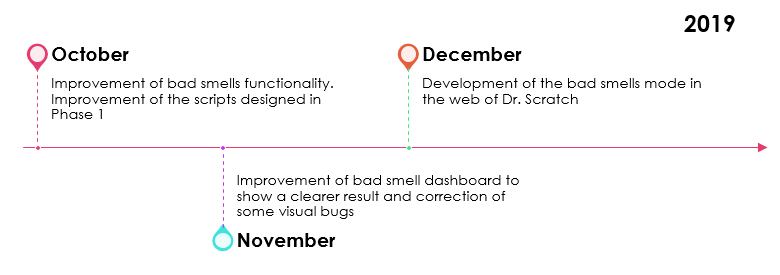
\includegraphics[width=12cm, keepaspectratio]{img/phase_3.png}
        \caption{Timeline planning for phase 3.}
        \label{fig:phase_3}
    \end{figure}
    
    \item Phase 4: Development of the bad smells model 
    
    \begin{figure}[h]
    \centering
        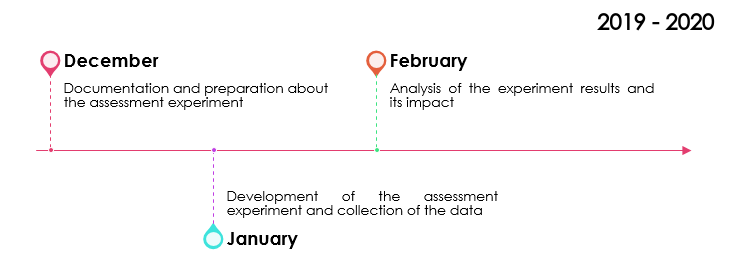
\includegraphics[width=12cm, keepaspectratio]{img/phase_4.png}
        \caption{Timeline planning for phase 4.}
        \label{fig:phase_4}
    \end{figure}
    
    \item Phase 5: Assessment experiment about the developed model
    
    \begin{figure}[h]
    \centering
        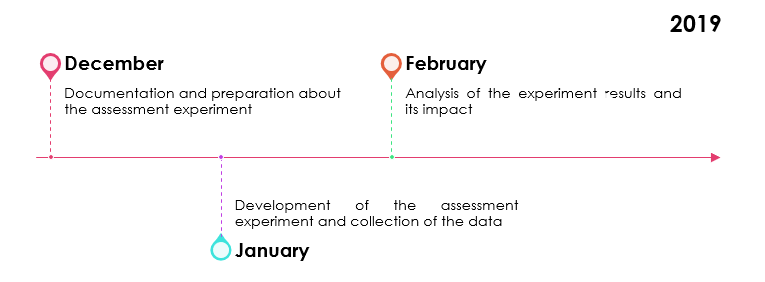
\includegraphics[width=12cm, keepaspectratio]{img/phase_5.png}
        \caption{Timeline planning for phase 5.}
        \label{fig:phase_5}
    \end{figure}
    
\end{itemize}
